\chapter{Conclusion}\label{chp:chapter5}
\section{Background}
Incoming freshmen struggle deciding which field of study they should enter. There are many computing fields and this can confuse new students who are interested in computing, especially because the fields are so closely related. For example, many students don't know the difference between computer science (CS), information systems (IS), and information technology (IT). It would be wonderful to have a simple way to determine which of these computing fields would best suit each student. How do these differences help us determine the right fit for incoming computing students?

One way to look at the differences among computing fields is to examine the students in each field~--- especially how they learn. CS, IS, and IT all focus on different areas of computing and each requires a different skill set. It seems like people in these fields have a preference for being taught differently. Is it possible to predict in which computing discipline an incoming freshman would succeed based on their learning style? Previous research has shown a correlation between learning preference and academic success, but does this correlation also exist for computing students?

In the 1970s, David Kolb developed a model to represent cognitive learning preference. His model works on a two-axis system: concrete experience (CE) versus abstract conceptualization (AC), and reflective observation (RO) versus active experimentation (AE). The \textit{x}-axis, AE$-$RO, differentiates between students who learn by doing or by seeing results, and those who prefer to learn by watching, listening, and taking their time. The \textit{y}-axis, AC$-$CE, differentiates between students who learn by reasoning and being rational, and those who prefer to trust their feelings.

The Association for Computing Machinery (ACM) has defined five disciplines in computing~(Shackelford, 2006): computer engineering, computer science (CS), information systems (IS), information technology (IT), and software engineering (SE). Although there is overlap between disciplines, each discipline is distinct. Computer engineering is focused on designing and building hardware. CS is concerned with the theoretical principles of computing, particularly the software. SE is focused on creating highly reliable software systems. IT solves general computer problems and focuses on systems integration. And IS fulfills an organizational need, but mostly from the management side.

Of the five computing disciplines, computer engineering is the least closely related to IT. SE is small in size nationwide and BYU doesn't even have an SE program. For these reasons, this study focused on CS, IS, and IT.

\subsection{Research questions}
\begin{itemize}
  \item How strong is the correlation between AC$-$CE and AE$-$RO, and major GPA among CS, IS, and IT students?
  \item How strong is the correlation between AC$-$CE and AE$-$RO, and student satisfaction among CS, IS, and IT students?
  \item Is there a correlation between major GPA and student satisfaction?
  \item What is the best multiple regression model to fit these correlations?
\end{itemize}

\subsection{Defining terms}
Kolb created the Experiential Learning Theory (ELT)~(Kolb, 2005a) and used it as the basis for his Learning Style Inventory (LSI) assessment. According to this theory, learning is more about the journey than the outcome. This is important because the ELT focuses on how ``[l]earning is the process of creating knowledge''~(Kolb, 2005a). This view is based on the Constructivist Theory of learning: that a learner must construct new knowledge: ``social knowledge is created and recreated in the personal knowledge of the learner''~(Kolb, 2005b). It is contrasted with the Transmission Model whereby ``pre-existing fixed ideas are transmitted to the learner''~(Kolb, 2005a). This might seem like a purely semantic difference, but there's an important distinction between constructivism and transmission which is important because the ELT and this research focus on learning as a process: it matters how students learn, not simply what they learn.

Satisfaction is how pleased a student is with their decision on their major. In order to be quantified, satisfaction was rated by the Academic Major Satisfaction Scale, developed and validated by Nuata. It asks if students are happy with their major, if they think of switching majors, and how they feel about their choice.

\subsection{Delimitations}
This research was limited to seniors because they have been exposed to myriad professors and courses, giving them a well-rounded view of the institution. Furthermore, this research was limited to CS, IS, and IT students at BYU because there are too many confounding variables to properly deal with other schools and their admissions processes in a study of this size.

This research did not look at the socioeconomic backgrounds of the students involved. It did not consider any social pressure students may receive to join a particular field.

\section{Literature review}
The literature review focused on studies already done on this topic, how previous studies in computing had incorporated cognitive theory, and what surveys to use to study cognitive theory among computing students, including criticism of the chosen surveys.

The initial literature review was to find studies related to cognitive or learning preference and how it bears on STEM students. Upon finding that there was bountiful research in the area, the literature review focused on finding studies on cognitive preference. Then, research was expanded to include studies on academic success.

\subsection{Lunt's \textit{Predicting Academic Success in Electronics}}
Barry Lunt's dissertation, \textit{Predicting Academic Success in Electronics}, was foundational. It performed the same research being performed here, but with an older version of the LSI, a focus on the electronics fields, and no focus on major satisfaction.

The purpose of Lunt's research was to determine if there was a correlation between learning style preference and academic success in electronics technology, electronics engineering technology, and electrical engineering. If there was a statistically significant correlation, then the LSI could be used as an accurate discriminator to help students choose in which electronics program they should enroll.

The students were randomly sampled and there was a participation rate of 45\%. Lunt asked: ``What are the best predictor variables for predicting academic success in electronics? Is abstract learning preference an effective discriminator between students in the three main types of electronics programs? What is the best multiple-regression model that can be derived for predicting success in each of the three types of electronics programs?''~(Lunt, 1996)

This rationale was persuasive because it focused on the difference between various majors in the same field and it was aimed at helping students determine which major to choose. Additionally, the Kolb LSI is a tested and validated tool for determining cognitive preference. Finally, the Experiential Learning Theory (ELT) on which the test is based fits right in line with the ideas behind this present research.

The multiple regression model presented found correlations which helped justify the need to expand this line of research to computing students.

\subsection{Other studies}
There were several non-cognitive studies~(Thomas, 2007; Elnagar, 2013; Ridgell, 2004; Ting, 2001) that were foundational in understanding the scope of research done in this field. Other studies focused on previous academic success~(Barlow-Jones, 2011; Golding, 2005; Ting, 2001; Campbell, 1984), programming or mathematics aptitude~(Nowaczyk, 1984; Evans, 1989), or other unrelated and non-cognitive models~(Barlow-Jones, 2011; Elnagar, 2013).

The most common non-cognitive tool used is the Non-Cognitive Questionnaire (NCQ); however Thomas found that ``none of the scales of the NCQ are adequate predictors of GPA or persistence in college''~(Thomas, 2007). Other non-cognitive tools included personality tests (e.g., Myers-Briggs Personality Type Indicator, 16 Personality Test), general knowledge tests (e.g., SAT, ACT), and work drive. In 2004, Ridgell studied these variables with great success ($p<0.01$) finding that the personality traits exam was found to statistically correlate with course grades and GPA. However, none of the tools Ridgell used were cognitively-based.

In the same vein, \textit{Predicting Academic Performance in the School of Computing \& Information Technology (SCIT)}~(Golding, 2005) looked at students' performance in first-year courses. This was useful because it looked at all courses a first year student takes, not just programming courses (as most studies did). The study used demographic information and aptitude score, as well as a student's overall performance in the program, to predict their future performance. However, the study did not look at college entrance exam scores or high school GPA. This research found that none of the entrance exams used~--- including the SAT~--- were good predictors for academic success. It also found that high school success in math and science and previous IS and IT classes were not good indicators for academic success. Mostly, this paper found that the then-current indicators for admission were incorrect and not statistically significant.

Historically, studies tried to determine academic success by a student's programming or math aptitude, using surveys like the Fennema-Sherman Mathematics Attitude Scale~(Nowaczyk, 1984) and the IBM Programmer Aptitude Test~(Hostetler, 1983), or even COBOL~(Nowaczyk, 1984) or FORTRAN~(Campbell, 1984) proficiency. However, these surveys were found to not be the most effective tools to determine future academic success with ``R-squares of less than 24 percent''~(Evans, 1989) used in the study.

\subsection{Why cognition?}
These studies take a non-cognitive approach to predicting academic success. Since previous studies have failed to look at cognition, it leaves a clear opportunity that this research can fill. Cognition might not be the right theory, but that needs to be addressed. Additionally, cognitive theory is a good candidate because it focuses on how students think and interpret information, which is key in understanding technical concepts.

\subsection{Criticism of the LSI}
In 1990, DeCoux surveyed cognitive research on nursing students that used the LSI. This was done in an effort to determine if the LSI was a trusted assessment tool. DeCoux's research showed ``a lack of significant relationships between learning style and other variables,'' adding further that ``studies undertaken specifically to investigate the measurement properties of the LSI reported major criticisms which seem to have been ignored.'' Throughout the survey, DeCoux found that the LSI was ``the most frequently used method of measuring learning styles'' even though there were ``numerous charges of serious instrument weakness,'' concluding that ``[c]ontinued use of the Kolb LSI... as an experiential technique is not recommended''~(DeCoux, 2016).

More recent research has shown that ``[d]ifferent personality traits... and academic motivation... were found to be independently associated with student learning strategies''~(Donche, 2013). This study, covering more than 1,100 undergraduate students, found that teaching strategy was hugely impactful because of ``the importance of students' personality and academic motivation'' which were found to ``partly explain''~(Donche, 2013) how students learn.

Despite these criticisms, the LSI has been widely used in previous research in this area and is still generally considered to be a valid assessment tool. Most of the studies looked at as part of this literature review did not have negative things to say about the LSI, although they were not looking into the tool's validity. For these reasons, we have decided to adopt the LSI as the learning style assessment tool.

\subsection{Criticism of cognition and learning styles}
Wang and others looked into the correlation between Biggs' constructive alignment and how it affected students' learning approaches. This research went off the basis that ``university students' learning approaches... are highly correlated with students' achievement of learning outcomes''~(Wang, 2013). However, it then noted that ``[s]uch a statement... was underpinned neither by qualitative nor quantitative empirical data.'' Their research showed that a more constructively-aligned teaching environment ``would lead students to adjust their learning approaches'' so they could learn more deeply ``despite their pre-existing individual differences
in the preferred learning approaches.'' Their research is important because it showed that learning preference, while not insignificant, could be forgone in order to learn deeply.

One of the main motivations fueling this research was the author's experience in IT and CS classes and how they so greatly differed. Because of the attitudes of the students in each major toward their courses and how the courses were taught, the author hypothesized that the cause of this schism was the learning styles of the students, so the author wished to pursue research in that realm.

\subsection{Conclusion on literature review}
The literature was severely lacking in cognitive studies in computing. Every study found took a non-cognitive approach, looked at programming aptitude, or tried to use previous academic success and aptitude tests to predict future academic success. Furthermore, the literature almost exclusively focused on CS with IT and IS being either completely overlooked or an afterthought. This study helps fill the gap in research by providing a look into the cognitive learning preferences of computing students. Since there is no clear way to successfully predict academic success in computing, this research will help fill that gap by exploring a new avenue to predict academic success in computing.

\section{Research methodology}
\subsection{Administration of tests}
To distribute the surveys, the author gained permission from professors to enter the classrooms of seniors in CS, IS, and IT. Once in the classroom, the author read the announcement script and distributed packets to each student. The packets contained a consent form, the demographic survey, the Kolb LSI, and the AMSS.

\subsection{Consent form}
The consent form was approved by BYU's Institutional Review Board (IRB). It contained information about the research and a place for students to sign granting access to their college transcripts. Additionally, the consent form contained information about the risks and benefits of the research, confidentiality, and what to do if a research subject had questions about the research.

\subsection{Kolb Learning Style Inventory (v3.1)}
The LSI is a twelve-question survey that takes between five and ten minutes to complete. The LSI charts cognition on a two-axis scale: concrete experience (CE) versus abstract conceptualization (AC), and reflective observation (RO) versus active experimentation (AE).

The LSI presents twelve, multiple-choice style questions. For instance, the question might start out: ``When I learn, I prefer to:'' and then gives four options, one from each quadrant (i.e., AC, AE, CE, RO). Students then mark the options one through four according to their personal preference. These scores and then added together to determine where the student's fall on each spectrum.

The responses were then totaled according to the algorithm provided by the Hay Group. The data was programmatically checked for integrity, and the results were input into a spreadsheet.

The LSI does not use the individual scores to plot the student's learning preference on the AC$-$CE and AE$-$RO axes so additional columns were added to compute these values. These values are best explained by example. Student 6 in the study scored CE=24, RO=33, AC=23, and AE=40 so the computed values are AE$-$RO=7 and AC$-$CE=-1. This student is pretty squarely in the middle of the graph. They don't lean heavily towards any of the cognitive preferences. By comparison, the author scored CE=48, RO=26, AC=21, and AE=25 so the computed values are AE$-$RO=-1 and AC$-$CE=-27. The author is moderate in the AE$-$RO axis~--- meaning he favors both active experimentation and reflective observation~--- but he is strongly in the abstract conceptualization camp. This might seem counter-intuitive because the author scored so high on CE, but is in the opposite (AC) end of the spectrum. This is because the individual scores aren't what matters: it is the calculated values (AE$-$RO and AC$-$CE) that define cognitive preference.

\subsection{AMSS}
The AMSS is composed of six questions rated on a 5-point Likert-type scale with 1 being ``strongly disagree'' and 5 being ``strongly agree.'' This scale has both positively and negatively worded statements, the negatively worded statements being reverse scored. These scores were input into their own columns on the respective student's row.

\subsection{Demographic information}
The demographic survey asked about the students' gender, age, ethnicity, marital status, and parents' highest education. The demographic information was added as columns to each student's existing scores with consistent spelling and punctuation. Each answer was input in separate columns.

\subsection{Participation rate}
Nulty discussed the differences between online and paper surveys, including their response rates and how to improve them, and how to improve evaluation~(Nulty, 2008). The most important part of this study for this research was a table listing the needed participation rates for various class sizes. However, the paper stated that the table is ``only a guide as it is based on the application of a formula derived from a theory that has random sampling as a basic requirement''~(Nulty, 2008).

From Nulty's research, it was found that a participation rate of 35-48\% was necessary for a 10\% sampling error and 80\% confidence level. The CS and IS senior classes were estimated by their respective departments to be 100 students each, so participation from 21 students was necessary for each major. The IT senior class was estimated at 40 students, requiring participation from 16 students.

\subsection{Major GPA}
Each student's major GPA was received from the Registrar's Office and input into the spreadsheet.

\section{Data analysis}
\subsection{Survey responses}
As discussed previously, a participation rate of 35-48\% was necessary for a 10\% sampling error and 80\% confidence level. This allows for inferences to be made on the population, not just the students sampled. The CS and IS senior classes were estimated by their respective departments to be one hundred students each, so participation from twenty-one students was necessary for each major. The IT senior class was estimated at forty students, requiring participation from sixteen students. Table~\ref{tab:c-response-rates} shows the amount of responses received compared to the total amounts needed.

\begin{table}[h!]
  \centering
  \caption{Response Rates of Various Majors}
  \label{tab:c-response-rates}
  \begin{tabular}{llllll}
    \toprule
    Major & Total seniors in major & Surveys needed & Surveys received & Response rate\\
    \midrule
    CS    & 100                    & 35             & 40               & 40\%\\
    IS    & 100                    & 35             & 2                & 2\%\\
    IT    & 40                     & 14             & 22               & 55\%\\
    \bottomrule
  \end{tabular}
\end{table}

There were many complications getting responses from IS students. IS seniors do not have a capstone or senior seminar class, so there was no common opportunity to reach them. Since the Learning Style Inventory (LSI) is copyrighted and licensed for hardcopy use, it couldn't be digitized for distribution. This made it difficult to get surveys into the hands of the IS students. After trying for a year to get surveys out and being stonewalled by significant distribution problems, only two surveys from IS students were completed, and those were only completed because those students were in an IT course in which the surveys were distributed. No additional surveys were returned from IS students. Because of the complications surrounding the IS responses, the IS results were not included in the analysis.

\subsection{What the LSI responses mean}
\subsubsection{Defining AC, CE, AE, and RO}
The terms abstract conceptualization (AC), concrete experience (CE), active experimentation (AE), and reflective observation (RO) are not really intuitive. Before diving into the statistical analysis, it will be helpful to more clearly define these terms. The following list contains statements to help define each of these terms~(Kolb, 1993):
\begin{enumerate}
  \item Abstract conceptualization
  \begin{enumerate}
    \item To learn, I'd rather think about ideas.
    \item I like to reason things out.
    \item I want to analyze things.
    \item I'm rational.
    \item I rely on my ideas.
  \end{enumerate}
  \item Concrete experience
  \begin{enumerate}
    \item Thinking about my feelings affects how I learn.
    \item I trust my feelings and intuition.
    \item I'm open to experiencing new things.
    \item I like to learn from personal relationships.
    \item I like being actively involved in the learning process.
  \end{enumerate}
  \item Active experimentation
  \begin{enumerate}
    \item I want to be doing.
    \item I like to work hard.
    \item I want to see results.
    \item Just let me try it out myself.
    \item I'm practical.
  \end{enumerate}
  \item Reflective observation
  \begin{enumerate}
    \item I prefer to watch and listen.
    \item When I learn, I'm quiet.
    \item I take my time when I learn.
    \item I'm reserved.
    \item I like to look at issues from different angles.
    \item I'm observant.
    \item I prefer to slow down and be careful.
  \end{enumerate}
\end{enumerate}

\section{Examining the data}
Before answering the research questions, it's necessary to look at the data, get a feel for it, and visualize it. To this end, I ran $t$-tests to see if there was a significant difference between CS and IT students in their AC$-$CE and AE$-$RO scores. Each of these were not statistically significant, with $p>0.05$. The AC$-$CE and AE$-$RO scores for CS and IT students are shown in a scatter plot in Figure~\ref{fig:c-cs-v-it-plot} where it can be seen that there does not appear to be any visible distinction between CS and IT for these results. This is interesting because it goes against what the literature previously discussed about the relationship between learning style preferences, \textit{viz}.: CS and IT should be distinct~(Kolb, 2005b).

\begin{figure}[!bhtb]
  \centering
  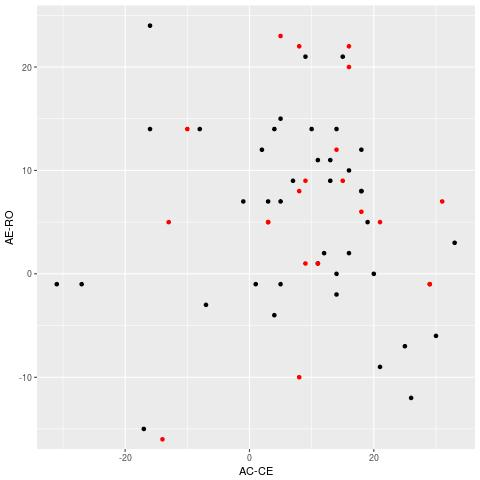
\includegraphics[width=0.7\textwidth]{figures/chapter4/cs-v-it-plot.jpg}
  \caption[AC$-$CE and AE$-$RO for CS and IT Students]{AC$-$CE and AE$-$RO for CS and IT Students}
  \label{fig:c-cs-v-it-plot}
\end{figure}

Next, I needed to know if the data was normally distributed in order to determine which correlation model to run. To determine if the data was normally distributed, I ran the Shapiro-Wilk test (note that $p<0.05$ here means that the data is \emph{not} normally distributed)). From this analysis, I can see that CS AC$-$CE was the only non-normal data with $p=0.0251$. These findings will be discussed alongside the first research question.

\section{Answering the research questions}
\subsection{How strong is the correlation between AC$-$CE and AE$-$RO, and major GPA among CS, IS, and IT students?}
Because all of these data points, except for CS AC$-$CE, are normally distributed, I was justified in using Pearson's correlation coefficient (also known as Pearson's $r$) to calculate the correlations. This data is summarized in Table~\ref{tab:c-pearsons} in which it can be seen that three of the four table entries were not statistically significant, while the IT major GPA and IT AE$-$RO, with $p=0.0202$, was statistically significant.

\begin{table}[!htbp]
  \centering
  \caption{Pearson's $r$}
  \label{tab:c-pearsons}
  \begin{tabular}{lll}
    \toprule
    Data                      & $p$-value & $r$ \\
    \midrule
    CS major GPA and CS AC$-$CE & 0.8177    & -0.0376 \\
    CS major GPA and CS AE$-$RO & 0.6704    & -0.0694 \\
    IT major GPA and IT AC$-$CE & 0.9727    & -0.0077 \\
    IT major GPA and IT AE$-$RO & 0.0202    &  0.4915 \\
    \bottomrule
  \end{tabular}
\end{table}

Since CS students' AC$-$CE results were not normally distributed, I ran Spearman's correlation coefficient to determine if there was a correlation between CS major GPA and CS AC$-$CE results. This resulted in $p>0.05$, but R gave a warning that Spearman's shouldn't be used for data with tied values. To account for the tied values, I then ran the correlation using Kendall's $\tau_b$ which also had $p>0.05$. With Pearson's $r$, Spearman's $\rho$, and Kendall's $\tau_b$ all having $p>0.05$, I am confident that there is no statistically significant correlation between CS major GPA and CS AC$-$CE results.

So, how strong is the correlation between AC$-$CE and AE$-$RO, and major GPA among CS, IS, and IT students? Because of these findings, I am unable to find a statistically significant correlation between any major GPA and a student's LSI results, except for IT major GPA and IT AE$-$RO (see Figure~\ref{fig:c-major_gpa_lm_plots}). In fact, IT AE$-$RO is so strongly correlated to IT major GPA that it has an $R^2=r^2=0.4915^2=0.2416$. This means that an IT student's AE$-$RO score is able to explain 24.16\% of their GPA. Interestingly, the AC$-$CE spectrum did not hold any statistically significant ($p>0.05$) effect on student GPA in CS or IT. This is interesting because Lunt found that AC$-$CE was the significant axis among electronics students~(Lunt, 1996).

\begin{figure}
  \centering
  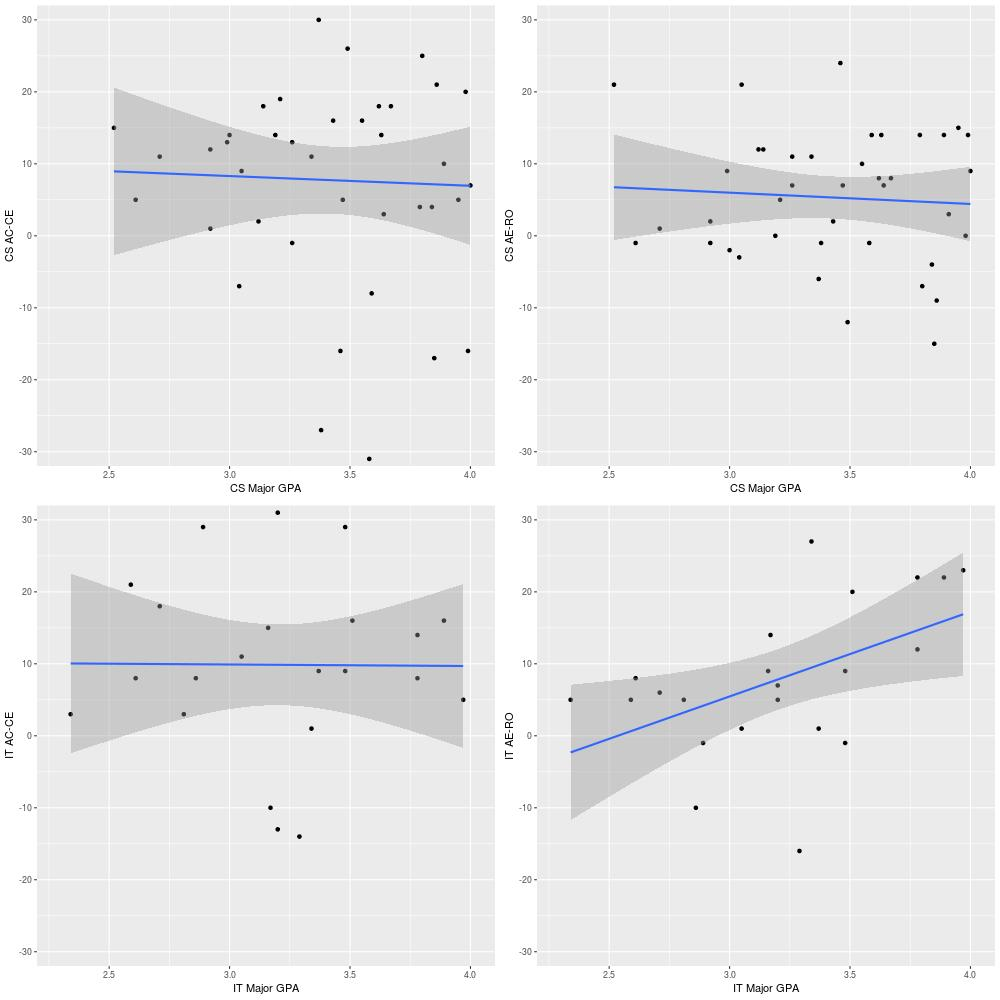
\includegraphics[width=1.1\textwidth]{figures/chapter4/major_gpa_lm_plots.jpg}
  \caption{Correlations Between Major GPA and LSI Results}
  \label{fig:c-major_gpa_lm_plots}
\end{figure}

\subsection{What is the best multiple regression model to fit these correlations?}
In order to estimate the relationship that AC$-$CE and AE$-$RO each have simultaneously, I developed several multiple regression models. I ran these models with standard errors computed with the Huber-White (HC1) robust standard error to account for the heteroskedasticity of the data. The most significant models can be seen in Table~\ref{tab:c-mr-models}. All three models used major GPA as the dependent variable, and compared that against the CS dummy variable (to determine if the student is a CS major), age, and parents' education level. Model~2 added AE$-$RO as a covariate, and Model~3 added AC$-$CE as a covariate.

% Table created by stargazer v.5.2 by Marek Hlavac, Harvard University. E-mail: hlavac at fas.harvard.edu
% Date and time: Sun, Jan 28, 2018 - 01:49:51 PM
\begin{table}[!htbp] \centering
  \caption{Multiple Regression Models}
  \label{tab:c-mr-models}
  \begin{tabular}{@{\extracolsep{5pt}}lccc}
    \toprule
     & \multicolumn{3}{c}{\textit{Dependent variable:}} \\
    \cline{2-4}
    \\[-1.8ex] & \multicolumn{3}{c}{Major GPA} \\
    \\[-1.8ex] & (1) & (2) & (3)\\
    \midrule
    CS dummy variable & 0.110 & 0.137 & 0.137 \\
    &  &  &  \\
    Age 25-29 & $-$0.196 & $-$0.177 & $-$0.177 \\
    &  &  &  \\
    Age 30-34 & $-$0.443 & $-$0.425 & $-$0.426 \\
    &  &  &  \\
    Age 35+ & $-$0.096 & $-$0.077 & $-$0.082 \\
    &  &  &  \\
    Parents education --- & $-$0.661 & $-$0.667 & $-$0.667 \\
    \hspace{2em}some college &  &  &  \\[+0.5em]
    Parents education --- & $-$0.631 & $-$0.534 & $-$0.534 \\
    \hspace{2em}undergraduate degree &  &  &  \\[+0.5em]
    Parents education --- & $-$0.680 & $-$0.602 & $-$0.601 \\
    \hspace{2em}graduate degree &  &  &  \\[+0.5em]
    Parents education --- & $-$0.157 & $-$0.080 & $-$0.080 \\
    \hspace{2em}post-graduate degree &  &  &  \\[+0.5em]
    AE.RO &  & 0.007 & 0.007 \\
    &  &  &  \\
    AC.CE &  &  & 0.0002 \\
    &  &  &  \\
    Constant & 3.976$^{*}$ & 3.828$^{*}$ & 3.826$^{*}$ \\
    & (0.159) & (0.110) & (0.103) \\
    \midrule
    Observations & 62 & 62 & 62 \\
    $R^{2}$ & 0.367 & 0.389 & 0.389 \\
    Adjusted $R^{2}$ & 0.272 & 0.283 & 0.269 \\
    Residual Std. Error & 0.364 (df = 53) & 0.361 (df = 52) & 0.365 (df = 51) \\
    F Statistic & 3.848$^{*}$ (df = 8; 53) & 3.681$^{*}$ (df = 9; 52) & 3.250$^{*}$ (df = 10; 51) \\
    \bottomrule
    \textit{Note:}  & \multicolumn{3}{r}{$^{*}p<0.05$} \\
  \end{tabular}
\end{table}

These models each have statistically significant ($p<0.05$) F statistics, so I reject the null hypothesis that that these groups of variables do not have a statistically significant joint effect. However, an interesting thing happens between models~2 and~3: adding the AC$-$CE covariate decreases the adjusted $R^2$. This means that while the model is still significant with that covariate, it doesn't explain the variance as well. Again, this goes against what Lunt found concerning AC$-$CE results~(Lunt, 1996). Because models~1 and~2 represent the best multiple regression models for this data, I chose to only plot those two (Figure~\ref{fig:c-mr_models_1_2}).

\begin{figure}
  \centering
  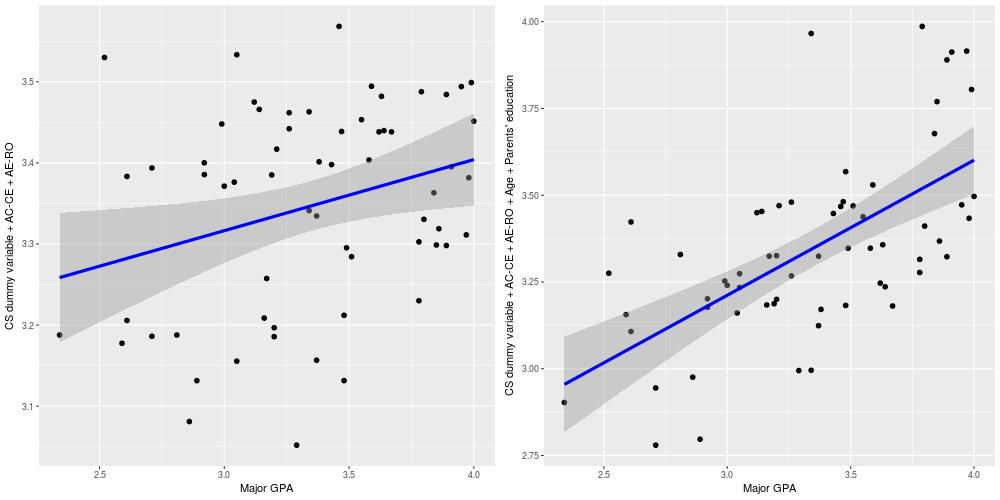
\includegraphics[width=1.1\textwidth]{figures/chapter4/mr_models_1_2.jpg}
  \caption{Multiple Regression Models 1 and 2}
  \label{fig:c-mr_models_1_2}
\end{figure}

Up to this point, I've only examined variables in groups, not individually. The linear hypothesis test compares the residual (error) sum of squares values against similar models. This way, I can check individual variables for a joint significance which will allow me to see if the variables can explain the deviance in the model. The null hypothesis is that each of these variables are 0. This test is important because removing unnecessary variables gives more power with this small of a dataset.

The model I ran used major GPA as the dependent variable, and compared it to the CS dummy variable, AE$-$RO, age, and parents education. This model had $p=1.266\times 10^{-10}$, so I reject the null hypothesis that these variables are not significant in explaining the variance in the data. This model reinforces the earlier, multiple regression findings.

\subsection{How strong is the correlation between AC$-$CE and AE$-$RO, and student satisfaction among CS, IS, and IT students?}
Nuata's AMSS, as enumerated in chapter 1, is graded on a five-point Likert-type scale with two of the responses being negatively scored. Two of the AMSS questions assume that students still have the option of changing their major, but once BYU students get beyond a certain credit threshold (well before their senior year), it becomes impossible for them to change majors. Because of this and the lack of variance among the responses, these questions were dropped from the analysis:
\begin{enumerate}
  \item I am strongly considering changing to another major.
  \item I would like to talk to someone about changing my major.
\end{enumerate}

I created a summary index of academic major satisfaction using the remaining AMSS variables and reverse coded the negatively-scored variables. In this summary index, the least satisfied value was a 4 and the most satisfied was a 20, with a mean of $18.10$ ($\sigma=2.2595$). This data is heavily left-skewed (see Figure~\ref{fig:c-amss_index_plot}). I believe the lack of response diversity led to the lack of correlations between student satisfaction and other factors.

\begin{figure}[!hbtp]
  \centering
  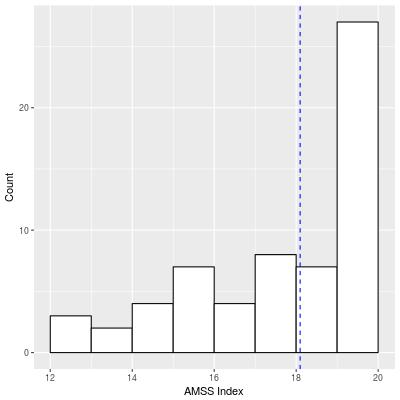
\includegraphics[width=0.5\textwidth]{figures/chapter4/amss_index_plot.jpg}
  \caption{AMSS Index Histogram}
  \label{fig:c-amss_index_plot}
\end{figure}

I then ran Pearson's $r$ for the data and found no statistically significant results (see Table~\ref{tab:c-amss_corr}), suggesting that there is no relationship between learning style and major satisfaction.

\begin{table}[!hbtp]
  \centering
  \caption{AMSS Correlations}
  \label{tab:c-amss_corr}
  \begin{tabular}{lll}
    \toprule
    $x$           & $y$        & $p$ \\
    \midrule
    AMSS index    & AC$-$CE    & 0.8563 \\
    AMSS index    & AE$-$RO    & 0.1059 \\
    CS AMSS index & CS AC$-$CE & 0.8134 \\
    CS AMSS index & CS AE$-$RO & 0.1237 \\
    IT AMSS index & IT AC$-$CE & 0.9566 \\
    IT AMSS index & IT AE$-$RO & 0.5147 \\
    \bottomrule
  \end{tabular}
\end{table}

\subsection{Is there a correlation between major GPA and student satisfaction?}
To determine if there is a correlation between major GPA and student satisfaction, I ran Pearson's $r$ against the data (Table~\ref{tab:c-satisfaction} and Figure~\ref{fig:c-major_gpa_amss_plots}) because all of the AMSS indices are normally distributed (with Shapiro-Wilk $p<0.05$).

\begin{table}[!htbp]
  \centering
  \caption{Major GPA and Student Satisfaction}
  \label{tab:c-satisfaction}
  \begin{tabular}{lll}
    \toprule
    $x$           & $y$          & $p$ \\
    \midrule
    AMSS index    & Major GPA    & 0.2127 \\
    CS AMSS index & CS major GPA & 0.3094 \\
    IT AMSS index & IT major GPA & 0.4532 \\
    \bottomrule
  \end{tabular}
\end{table}

\begin{figure}[!hbtp]
  \centering
  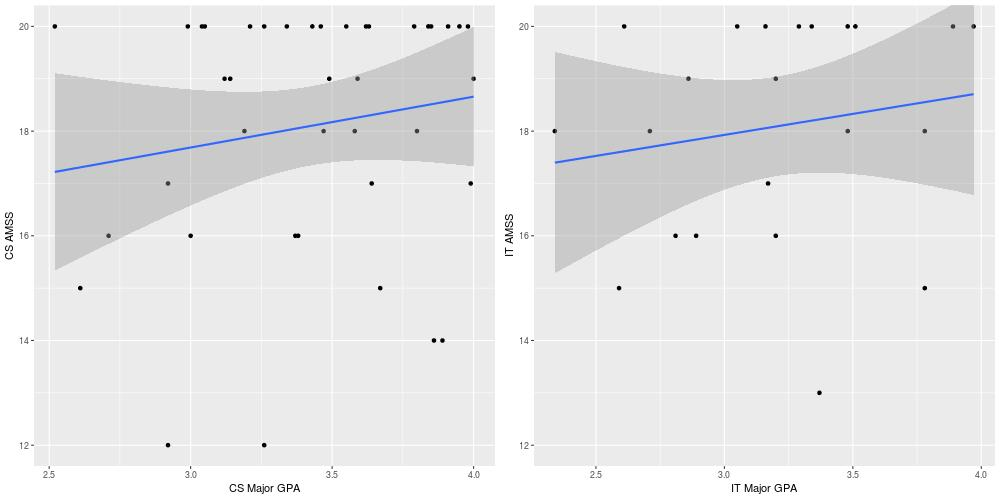
\includegraphics[width=1.05\textwidth]{figures/chapter4/major_gpa_amss_plots.jpg}
  \caption{Major GPA and Student Satisfaction Correlations}
  \label{fig:c-major_gpa_amss_plots}
\end{figure}

The Pearson correlation coefficient for each major GPA and the corresponding AMSS index are $p>0.05$, so I am unable to say that there is a significant correlation between the two.

\section{Demographics}
Unfortunately, I was unable to use the full set of demographic variables collected from students as covariates because there was not enough variance among the sample group. The students were almost entirely white and male (88\% for both). Looking at the relationship between marital status and its effect on major GPA and satisfaction had a multiple $R^2$ of $0.07$, meaning that marital status was only able to explain 7\% of the variance in major GPA and satisfaction. While students were equally divided in marital status (31 single, 31 married), there was no relationship between marital status and any other factor. The multiple regression analysis for the demographic information, calculated with robust standard error, is summarized in Table~\ref{tab:c-demographics}.

% Table created by stargazer v.5.2 by Marek Hlavac, Harvard University. E-mail: hlavac at fas.harvard.edu
% Date and time: Sun, Jan 28, 2018 - 05:36:26 PM
\begin{table}[!htbp] \centering
  \caption{Demographic Regression Analysis}
  \label{tab:c-demographics}
  \begin{tabular}{@{\extracolsep{5pt}}lc}
    \toprule
     & \multicolumn{1}{c}{\textit{Dependent variable:}} \\
    \cline{2-2}
    \\[-1.8ex] & AMSS index \\
    \midrule
    Major GPA & 1.088 \\
    &  \\
    CS dummy variable & $-$0.276 \\
    &  \\
    Age 25-29 & $-$0.536 \\
    &  \\
    Age 30-34 & $-$0.034 \\
    &  \\
    Age 35+ & 0.723 \\
    &  \\
    Gender~--- female & $-$3.251 \\
    &  \\
    Gender~--- male & $-$3.275 \\
    &  \\
    Constant & 18.072$^{*}$ \\
    & (2.230) \\
    \midrule
    Observations & 62 \\
    $R^{2}$ & 0.070 \\
    Adjusted $R^{2}$ & $-$0.051 \\
    Residual Std. Error & 2.316 (df = 54) \\
    F Statistic & 0.578 (df = 7; 54) \\
    \bottomrule
    \textit{Note:}  & \multicolumn{1}{r}{$^{*}p<0.05$} \\
  \end{tabular}
\end{table}

\subsection{Research questions summarized}
\subsubsection{How strong is the correlation between AC$-$CE and AE$-$RO, and major GPA among CS, IS, and IT students?}
IT AE$-$RO is strongly correlated to IT major GPA with $R^2=0.2416$. This means that an IT student's AE$-$RO score is able to explain 24.16\% of their GPA.

\subsubsection{How strong is the correlation between AC$-$CE and AE$-$RO, and student satisfaction among CS, IS, and IT students?}
I found no statistically significant results, suggesting that there is no relationship between learning style and major satisfaction.

\subsubsection{Is there a correlation between major GPA and student satisfaction?}
The Pearson correlation coefficient for each major GPA and the corresponding AMSS index are $p>0.05$, so I am unable to say that there is a significant correlation between the two.

\subsubsection{What is the best multiple regression model to fit these correlations?}
The best multiple regression model I found used major GPA as the dependent variable, with the CS dummy variable, age, parents' education level, and AE$-$RO as covariates.

\subsection{Future work}
First and foremost, this research needs to be repeated for IS students at BYU. It was unfortunate that so little data was able to be gathered, and adding that dataset to this line of research is necessary, especially in light of the correlations that were found.

This research did not independently evaluate the AC$-$CE and AE$-$RO environments for the individual courses. That would amount to a large amount of low-level work which was outside the scope of this study. However, it would be interesting to see how each of the classes stack up in their cognitive styles.

Since IT students take so many CS classes and tend to do poorly in them, this research should be repeated to omit the CS classes from the IT major GPA and see if and how that affects correlations.

The multiple regression models that I first developed were based on the calculated differences (i.e., AC$-$CE and AE$-$RO) and not on the decomposed variables. The rest of the multiple regression models were exploratory. Future research should be more explicit in the data analysis methods that will be used before beginning the data analysis.

From the research, it seems like there are two main camps regarding teaching based on learning style: worry about it or don't worry about it. Some research has shown that when students are taught according to their preferred learning style, they learn better~(Vizeshfar, 2017; Donche, 2013). Others have shown that students adapt to how courses are taught regardless of learning style~(Wang, 2013). This study examined if a student's cognitive learning preference was a factor in which computing discipline they should explore. However, this angle helps perpetuate the \textit{status quo} by advising students to only go into a field where a majority of their classmates will have similar cognitive preferences. Instead, research should be done into each field's cognitive approach and determining if that approach is the best way to instruct students in that field.

There is a lot of noise surrounding whether or not the Kolb Learning Style Inventory (LSI) is a valid tool. Many articles have used it and said that it's a tried and true method. However, DeCoux shows ``numerous charges of serious instrument weakness'' and states conclusively that ``[c]ontinued use of the Kolb LSI in nursing research or as an experiential technique is not recommended''~(DeCoux, 2016). There is a need for good research showing whether or not the LSI is a trusted method, and if it is not, its weaknesses should be explored. That research needs to be disseminated in order to persuade future researchers in their methodology.
